\section[协方差与最优权]{协方差与最优权\\Covariances and Optimal Weights}
科学计算的一部分是统计计算,如果我们研究如何从输入值b计算输出值$\hat{x}$,我们也必须研究如何估计从b的可靠性中得到$\hat{x}$的可靠性。可靠性通过方差和协方差来评估,所以我们通过输入误差(在b中)的协方差矩阵$\Sigma$得到输出误差(在x中)的协方差矩阵$P$。

这个漂亮的公式$P=(A^TCA)^{-1}=(A^T\Sigma^-1A)^{-1}$给出那些协方差值。矩阵P显示了被估计的$\hat{x}$的可靠性或不可靠性,注意到P不依赖于明确的b(实验数据),它只依赖于A和协方差阵(实验装置)。P的含义提前讲述了这个实验多么好。

这是一个“数据世纪”,可靠性是一个重要的科学问题。这一章节将更加深入地叙述最小二乘,接着之前章节已经做好的铺垫$A^TA\hat{x}=A^Tb$。这一算法将x与统计学和应用的数学的其他部分联系起来,可靠性分析是试验和仿真的关键性环节。

首先,我们解释方差和协方差,然后我们展示为什么加权矩阵(中间步骤在框架中)是输入协方差矩阵的逆矩阵,最后我们提出如何在不重复计算先前b的情况下使用新的输入值(新的观测值)。当我们在$Au\approx b$中加入新的方程时,这就是最小二乘,当x和它的统计在每一步都变化时,$\hat{x}_i$的递归式和协方差矩阵$P_i$变为著名的卡尔曼滤波。
	
	\subsection[概率分布]{概率分布\\Probability Distributions}
	这有三个概率分布的例子。例1(盒形图)和例3(钟形图)具有连续变量,在x点的曲线高度是概率密度$p(x)$,样品落在$x$和$x+dx$之间的概率为$p(x)dx$,$p(x)$关于0对称,保证了误差的期望值为$m=E\{M\}=0$。每项误差以它的概率定权,平均值为0(因为当$p(-x)=p(x)$时,$-x$平衡于$x$),这些误差有零均值。
	
	例2中,我们记录n次公平地投掷硬币正面出现的次数为M,M为离散的随机变量,概率$p_0,...,p_N$加起来为1。期望值$E\{M\}$(正面出现的平均值)为平均值N/2。强大的大数定律提出,当我们不停的投掷硬币时,那么M/N与1/2的差值将会无限趋近于0。
	
	正态分布(钟形高斯)是迄今为止最常见的分布,重复实验的平均值令中心极限定理更加自然和有意义。
	
	均匀分布   \quad 假设每一个测量值舍入到最近的整数,6.5到7.5之间的数全部给定7,误差e在-0.5到0.5之间,在这个区间内的误差具有同样的可能性(这解释为均匀分布),误差e落在0到$\frac{1}{4}$的概率为$\frac{1}{4}$:
	
	$p(x)=1$      \qquad $x<$误差$<x+dx$的概率为:dx
	
	$\int p(x)dx$   \qquad $-\frac{1}{2}<e<\frac{1}{2}$的总概率为:$\int^{\frac{1}{2}}_{-\frac{1}{2}}dx=1$
	
	平均值m         \qquad 误差期望值为:$E\{e\}=\int^{\frac{1}{2}}_{-\frac{1}{2}}xp(x)dx=0$
	
	方差$\sigma^2$  \qquad 误差平方期望值为:$\int^{\frac{1}{2}}_{-\frac{1}{2}} x^2 p(x)dx=\frac{1}{12}$
	
	二项式分布  
	\quad 每次抛掷一个均匀的硬币,正面朝上的概率为$\frac{1}{2}$。抛掷3次硬币,每次都是正面朝上的概率为$\frac{1}{1}^{3}=\frac{1}{8}$,出现两次正面一次反面的概率为$\frac{3}{8}$,共有三种排列:THH、HTH、HHT。$\frac{1}{8}$和$\frac{3}{8}$是$(\frac{1}{2}+\frac{1}{2})^{3}=1$的一部分:
	
	总概率:
	\begin{equation*}
	(\frac{1}{2})^{3}+3(\frac{1}{2})^{3}+3(\frac{1}{2})^{3}+(\frac{1}{2})^{3}=\frac{1}{8}+\frac{3}{8}+\frac{3}{8}+\frac{1}{8}=1
	\end{equation*}
	正面朝上的平均数为1.5,用这四个概率作为权重:
	
	平均值:
	\begin{equation*}
	m=(3heads)\frac{1}{8}+(2heads)\frac{3}{8}+(1head)\frac{3}{8}+0=\frac{12}{8}heads
	\end{equation*}
	N次抛掷硬币中M次出现正面的概率是多少?我们再一次看这个条件$(\frac{1}{2}+\frac{1}{2})^{N}$,可以看到M次正面朝上N-M次反面朝上的概率$p_M$涉及到赌徒了解并喜爱的二项式系数$\begin{pmatrix}
		N \\ M
	\end{pmatrix}$=“N次里面选出M次”。
	
	二项式分布
	\begin{equation*}
	p_M = \frac{1}{2^N}
	\begin{pmatrix}
	N \\ M
	\end{pmatrix}
	=\frac{1}{2^N}\frac{N!}{M!(N-M)!}
	\end{equation*}	
	\begin{figure}
		\centering
		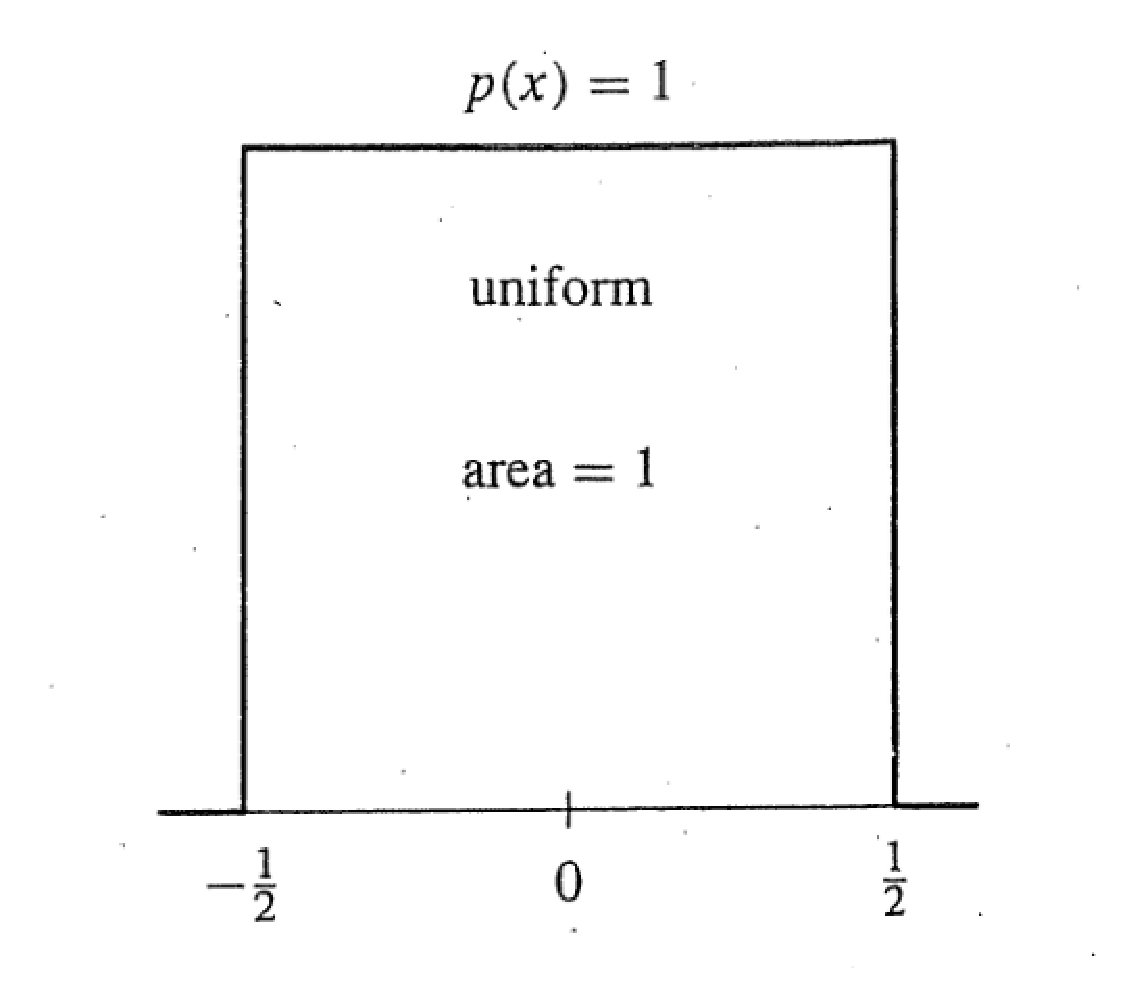
\includegraphics[width=0.7\linewidth]{TeX_files/Part02/chapter04/image/4-2}
		\caption{-1/2到1/2之间的相等概率}
		\label{fig:4-2}
	\end{figure}	
	由图\ref{fig:4-2}可知,总概率为:$p_0+...+p_N=(\frac{1}{2}+\frac{1}{2})^N=1$。正面朝上的期望值为$\bar{M}=0p_0+2p_1+...+Np_N=N/2$,这来自于常识。
	
	由于平均值为N/2,我们因此得到距离平方,它的期望值(平方距离?概率)是方差$\sigma^2$:
	\begin{equation*}
	\sigma^2=(0-\frac{N}{2})^2p_0 + (1-\frac{N}{2})^2p_1 + ...+ (N-\frac{N}{2})^2p_N
	\end{equation*}
	
	这一结果为$\sigma^2=N/4$,标准差为方差的平方根$\sigma=\sqrt{N}/2$。在平均值周围测量传播。
	
	一个不均匀的硬币正面朝上概率为p,反面朝上概率为$q=1-p$,正面朝上的平均值为$m=pN$,方差为$\sigma^2=pqN$。
	
	正态分布 \quad 这种“高斯”分布是最重要的,它总是在我们结合大量相同且独立的样本(例如投掷硬币)时出现,通过测量平均值N/2和以标准差$\sigma=\sqrt{N}/2$来区分使正面朝上次数M标准化。
	
	正面朝上次数标准化:
	\begin{equation*}
	x=\frac{1}{\sigma}(M-mean)=\frac{2}{\sqrt{N}}(M-\frac{N}{2})
	\end{equation*}
	
	随着N的增加,x可能的输出值将落在$-\infty$到$\infty$整个直线上,中心极限定理提出,这些随机变量x的概率接近高斯分布,正面朝上次数标准化的概率在一个介于$x$到$x+dx$的小区间中,为:
	\begin{equation}
	p(x)dx=\frac{1}{\sqrt{2\pi}}e^{-x^{2}/2}dx
	\end{equation}
	总概率为:
	\begin{equation*}
	\int^{\infty}_{-\infty}p(x)dx=1	
	\end{equation*}
	\begin{figure}
		\centering
		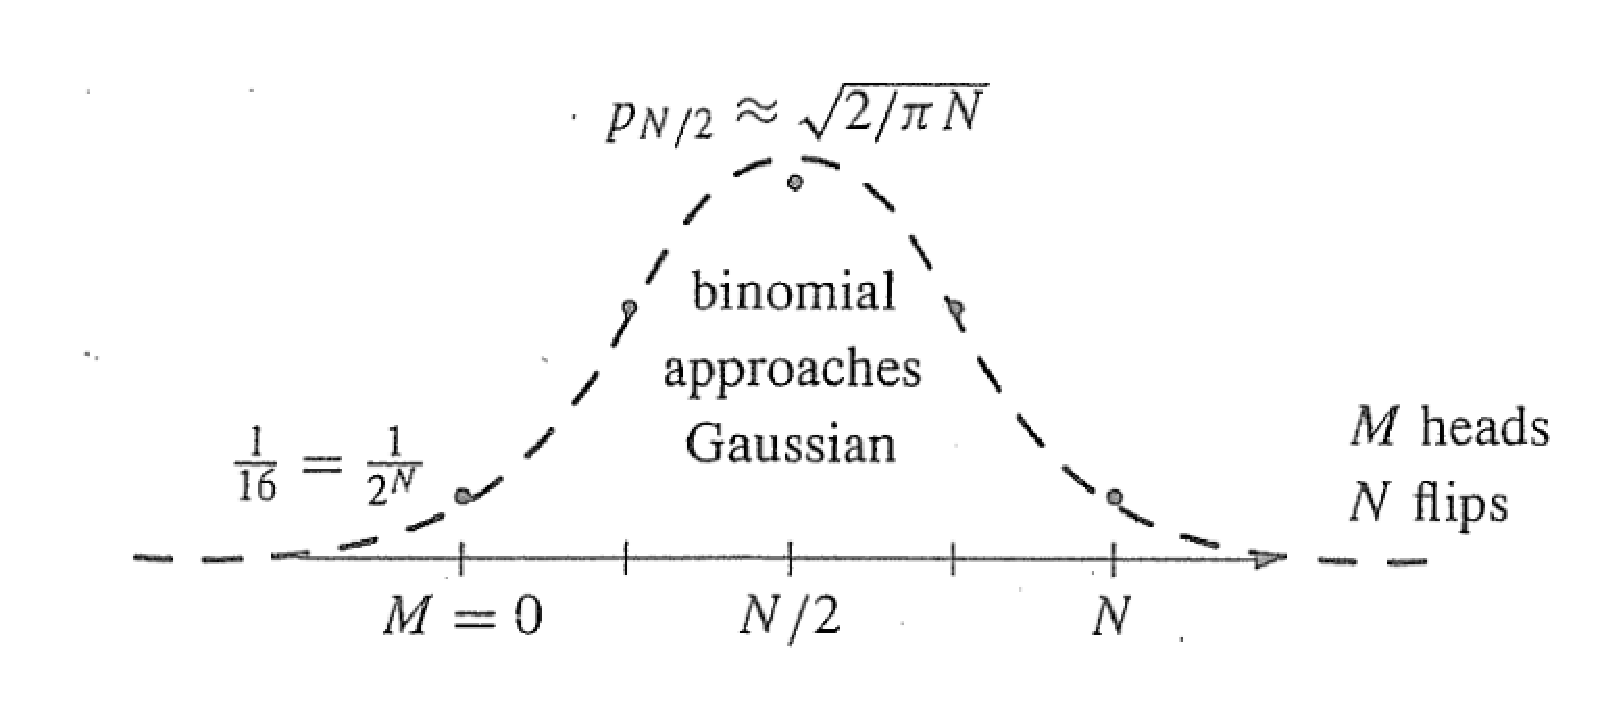
\includegraphics[width=0.7\linewidth]{TeX_files/Part02/chapter04/image/4-3}
		\caption{}
		\label{fig:4-3}
	\end{figure}
	
	\quad二次项分布$p=(1,4,6,4,1)/16$加上1来自于$\begin{pmatrix}
	N \\ M
	\end{pmatrix}/2^N$当N=4时,这接近于高度为$\sqrt{2/\pi N}$,和方差为$\sigma^2=N/4$的高斯分布。
	
	因素$\sqrt{2\pi}$确保了总概率为。在图\ref{fig:4-3}中,$e^{-x^{2}/2}$图是著名的钟形曲线图,它的积分$F(x)$给出了所有不超过x结果的累积积分,由对称性可知,x的平均值为$\int
	xp(x)dx=0$,方差为$\int x^2p(x)dx=1$。MATLAB的randn使用的是正态分布,但是rand的输出是均匀分布。
	
	均值为m=0(更多时候写成$\mu=0$),方差$\sigma^2=1$的标准正态分布是通过标准化正面朝上次数产生的,非标准正态分布的中心为均值$\mu=\int xp(x)dx$,钟形的宽度为方差$\sigma$:
	\begin{equation}
	p(x)=\frac{1}{\sqrt{2\pi}\sigma}e^{-(x-\mu)/2\sigma^{2}}
	\end{equation}
	有
	\begin{equation*}
	\int p(x)dx=1 \qquad \int(x-\mu)^2p(x)dx=\sigma^2
	\end{equation*}
	
	当你阅读到一个民意调查结果时,报纸总是给出平均值,也经常报道出一个从$\mu-2\sigma$到$\mu+2\sigma$的区间,样品在此范围内的概率约为$\textdiscount95$。从图4.5(方差为1)可以看出,概率函数p(x)下方约$\textdiscount95$的面积介于$-2\sigma$到$+2\sigma$,面积以“累积概率”$F(x)$,即$p(x)$积分所体现,定积分$F(2)-F(-2)$接近于0.95,错误的可能性小于$2\sigma$。
	
	多元正态分布  \quad  对于m个随机变量,概率密度函数由$p(x)$变为$p(b)=p((b_1,...,b_m)$,零均值的正态分布由一个整数$\sigma^2$所约束,而p(b)由一个m*m的正定矩阵$\Sigma$所约束,这就是它的协方差阵和行列式$|\Sigma|$:
	\begin{equation*}
	p(x)=\frac{1}{\sqrt{2\pi}\sigma}e^{-x^2/2\sigma^2}
	\end{equation*}
	因为
	\begin{equation*}
	p(b)=\frac{1}{(2\pi)^{m/2}|\Sigma|^{1/2}}e^{-b^{T}\Sigma^{-1}b/2}
	\end{equation*}
	
	P(b)在m维空间上的积分总概率为1。bp(b)的积分给出全为零的均值$b_1,...,b_m$,$bb^Tp(b)$的积分为多元正态分布给出了协方差阵$\Sigma$,这种积分降到出现在指数中的矩阵。
	
	假如$\Sigma=I$,指数$-b^T\Sigma^-1b/2$正好是和$-(b^2_1+...+b^2_m)/2$,所以分布$p(b_1,...b_m)$是通过m分割一维正态分布所产生的,正如我们期望的当$\Sigma=I$。
	
	现在我们需要理解协方差$\sigma_ij$和矩阵$\Sigma$。
	
	\subsection[协方差矩阵]{协方差矩阵\\The Covariance Matrix}
	同时做m个不同的实验,它们可能是独立的,或者它们之间有某种相关性。现在每个测量值x是一个向量,包含从每个实验输出的$x_i$,我们想更多地讲述一下协方差。
	
	如果我们平均观测距离$e_i$,每个误差$e_i$均值为0。如果两个误差$e_i$和$e-j$是独立的(它们之间没有相关性),则$e_ie_j$均值也为零。但是,如果测量由同一观察者几乎在同一时间进行,误差$e_i$和$e_j$可能具有相同的符号和大小,在m次实验中的误差可能具有相关性。从m个相邻接收机获得的定位误差极有可能具有相关性,$e_ie_j$的平均值为协方差$\sigma_ij$:
	\begin{equation}
	\sigma_ij=\sigma_ji=E\{e_ie_j\}=e_i*e_j
	\end{equation}
	
	这是协方差矩阵$\Sigma$的项$(i,j)、(j,i)$,对角线上的项($(i,i)$为方差$\sigma^2_i$。
	
	一种估计数字$\sigma_ij$的方法是多次进行实验,一份民意调查可能会发现一对夫妻的回复是相关的,可能是正相关,也可能是负相关。回复可能相同(协方差大于0)或者相反(协方差小于0)。从数据中估计方差和协方差是一个重要且不平凡的问题。
	
	如果每个实验进行m次,输出向量$x^1,x^2,...,x^m$提供样本均值$\bar{\mu_i}$和样本方差$\bar{\sigma_i}^2$协方差$\bar{\sigma_{ij}}$。当我们不知道真实的$\mu_i,\sigma^2_i,\sigma_{ij}$时,这是一个自然的选择。样本值:
	\begin{equation}
	\bar{\mu_i}=\frac{x^1_i+...+x^m_i}{m}  \qquad \bar{\sigma_ij}=\frac{(x^k_i-\bar{\mu_i})(x^k_j-\bar{\mu_j})}{m-1}
	\end{equation}
	
	当“一个自由度被使用”在$\mu_i$中,注意要除以m-1。
	
	例4.2 \quad 假定同样的标量变量m个观测值为$b_1,...,b_m$,我们想要证明加权平均$\hat{x}$和它的方差如下:
	\begin{equation}
	\hat{x}=\frac{u^TCb}{u^TCu}  
	\qquad \hat{\sigma}^{2}_{\hat{x}}=\frac{1}{(m-1)}\frac{\hat{e}^TC\hat{e}}{u^TCu}
	\end{equation}
	这里我们介绍$\hat{e}=b-A\hat{x}$和向量$u^T=[1 1 ... 1]$,m个观测方程$x_i=b_i-e_i$可以从矩阵$Ax=b-e$和$A=u$写出:
	\begin{equation*}
	\begin{bmatrix}
	1 \\ 1 \\ \vdots \\1
	\end{bmatrix}
	x=
	\begin{bmatrix}
	b_1 \\ b_2 \\ \vdots \\ b_m
	\end{bmatrix}
	-
	\begin{bmatrix}
	e_1 \\ e_2 \\ \vdots \\ e_m
	\end{bmatrix}
	\end{equation*}
	正常方程$A^TCAx=A^TCb$为:
	\begin{equation*}
	\begin{bmatrix}
	1 & \dots & 1
	\end{bmatrix}
	\begin{bmatrix}
	c_1 & \quad  &\quad \\
    \quad & \ddots & \quad \\
	\quad & \quad  & c_m
	\end{bmatrix}
	\begin{bmatrix}
	1 \\ \vdots \\ 1
	\end{bmatrix}
	\hat{x}=
	\begin{bmatrix}
	1 & \dots & 1
	\end{bmatrix}
	\begin{bmatrix}
	c_1 & \quad  &\quad \\
	\quad & \ddots & \quad \\
	\quad & \quad  & c_m
	\end{bmatrix}
	\begin{bmatrix}
	b_1 \\ \vdots \\ b_m
	\end{bmatrix}
	\end{equation*}
	
	$\Sigma^{m}_{i=1}c_i\hat{x}=\Sigma^{m}_{i=1}c_ib_i$和答案是加权平均值$\hat{x}$:
	\begin{equation}
	\hat{x}=\sum_{i=1}^{m}c_ib_i / \sum_{i=1}^{m}c_i=u^TCb/u^TCu
	\end{equation}
	
	例4.3 \quad 最后我们对相关性理论做了初步勘验和其最终影响。假设我们已经观测了一个给定的距离两次,结果为$b_1=100m$,$b_2=102m$,最小二乘估计的长度为$\hat{x}$,如果C=I,那么平均值$\hat{x}=101m$。如果C是对角阵,我们得到$b_1<\hat{x}<b_2$,当$c_1\textrightarrow \infty $我们得到$\hat{x}=b_1$,当$c_2\textrightarrow \infty$,我们得到$\hat{x}=b_2$,对角阵C(没有相关性)的最小二乘结果总是介于最小和最大观测值之间。
	
	如果两个相关的观测值情况急剧变化,我们对着两个观测值仍有$A^T=\begin{bmatrix} 1 & 1\end{bmatrix}$假设逆方差矩阵为:
	\begin{equation*}
	\begin{bmatrix}
	5 & 2 \\ 2 & 1
	\end{bmatrix}^{-1}
	=
	\begin{bmatrix}
	1 & -2 \\ -2 & 5
	\end{bmatrix}
	=C
	\end{equation*}
	
	现在$A^TCA=2,A^TCb=206$,因此$\hat{x}=103>b_2$。一个很强的正相关结合$b_2$一个大权重导致$\hat{x}>b_2$,这在独立观测值中是不可能发生的。在第6.5节中,我们将展示任意协方差阵如何导致任意最小二乘结果,你可以运行M文件。
	
	假设我们知道这两个误差的真实联合分布,介于$x$和$x+dx$之间的误差$e_1$,$y$和$y+dy$之间的误差$e_2$的概率为$p(x,y)dxdy$,当平均值x和y都不为0,用$x-\bar{x}$和$y-\bar{y}$代替x和y,协方差为:
	\begin{equation}
	\sigma_12=\iint xyp(x,y)dxdy
	\end{equation}
	对于独立误差,$p(x)p(y)$产生$p(x,y)$,双重积分是$\sigma_12=0$:
	\begin{equation*}
	\sigma_12=\iint xyp(x)p(y)dxdy=\int xp(x)dx\int yp(y)dy=(0)(0)
	\end{equation*}
	当误差e独立时,协方差为0,$\Sigma$变为对角矩阵,这种情况是目前为止最为简单的计算。
	
	$\Sigma$的对角线上的项为方差$\sigma^2$,那些是$e^2_i$的平均值,必然为正。这是一种很好的方式把所有的方差和协方差放在一个矩阵公式中,让列向量e与行向量$e^T$相乘,方差矩阵为:
	\begin{equation}
	\Sigma=E\{ee^T\}=E
	\begin{Bmatrix}
	e^2_1 & e_1e_2 & \quad & e_1e_m \\
	\quad &\quad   & \dots & \quad  \\
	e_me_1&e_me_2  & \dots &e^2_m
	\end{Bmatrix}
	\end{equation}
	
	$ee^T$的平均值为$\Sigma$,这个矩阵总是对称的,几乎总是正定的!(当误差的固定组合为零,矩阵总是半定的,这表明是一个失败的实验)接下来关键的步骤是展现C应该被选为$\Sigma^{-1}$。
	
	从协方差的$p_{ij}=\sigma_{ij}/\sigma_i\sigma_j$知,“相关系数”是无量纲的(栉比鳞次的),相关系数矩阵的对角项为$\sigma^2/\sigma^2=1$。
	
	\subsection[加权矩阵$C=\Sigma^{-1}$]{加权矩阵$C=\Sigma^{-1}$ \\ The Weighting Matrix $C=\Sigma^{-1}$}
	我们将表明选择$C=\Sigma^{-1}$将最大限度的减少$\hat{x}$中的预期平方误差,从$\hat{x}$的正规方程开始,它在$\hat{x}=Lb$中产生了矩阵L。
	\begin{equation}
	A^TCA\hat{x}=A^TCb
	\end{equation}
	给出
	\begin{equation*}
	\hat{x}=(A^TCA)^{-1}A^TCb=Lb
	\end{equation*}
	注意L乘以A,即$(A^TCA)^{-1}A^TC$乘以A,给出$LA=I$。
	
	我们想让协方差矩阵(所有的方差和协方差)输出误差向量为$x-\hat{x}$,既然$LA=I、\hat{x}=Lb$,这个输出误差为$-Le$,输出误差为:
	\begin{equation}
	x-\hat{x}=LAx-Lb=-L(b-Ax)=-Le
	\end{equation}
	
	(4.16)中m方程,矩阵$ee^T$产生所有的$e_ie_j$,类似地,我们使列向量$x-\hat{x}$乘以它的转置得到n*n的矩阵,误差$x-\hat{x}$的协方差矩阵P为平均值(期望值)$(x-\hat{x})(x-\hat{x})^T$,协方差为:
	\begin{equation}
	P=E\{(x-\hat{x})(x-\hat{x})^T\}=E\{(Le)(Le)^T\}=LE\{ee^T\}L^T=L\Sigma L^T
	\end{equation}
	这是我们的关键方程,第二步使用(4.18),唯一的新步骤是将常数矩阵L和$L^T$带到期望值$E\{ee^T\}$和或积分的外面。这是标准过程,被称为“方差传播”,现在我们已经准备好减小P,通过在矩阵L中选择最佳的C,这是结果。
	
	在$LA=I$的要求下,当C(在L中使用)为$C=\Sigma^{-1}$时,协方差矩阵$P=L\Sigma^{-1}L^T$尽可能小,这给出了最佳线性无偏估计$\hat{x}$(BLUE),误差$x-\hat{x}$的协方差矩阵简化,当$C=\Sigma^{-1}$时,输出矩阵为:
	\begin{equation}
	P=E\{(x-\hat{x})(x-\hat{x})^T\}=(A^T\Sigma^{-1}A)^{-1}
	\end{equation}
	
	使用矩阵L中的$C=\Sigma^{-1}$检查(4.20),这个选择给出了一个特性$L=L^*$:
	\begin{equation}
	P=L^*\Sigma L^{*T}=((A^T\Sigma^{-1}A)^{-1}A^T\Sigma^{-1})\Sigma(\Sigma^{-1}A(A^T\Sigma^{-1}A))=(A^T\Sigma^{-1}A)^{-1}
	\end{equation}
	
	C的选择不同,则L不同,我们仍有$LA=I$和$L^*A=I$,因此$(L-L^*)A=0$,为了显示远离$C=\Sigma^{-1}$而产生一个更大的协方差矩阵P的变化,写出$L=L^*+(L-L^*)$,为这个不同的选择计算$P=L\Sigma L^T$:
	\begin{equation}
	P=L^*\Sigma L^{*T} + (L-L^*)\Sigma L^{*T} + L^*\Sigma(L-L^*)^T + (L-L^*)\Sigma(L-L^*)^T
	\end{equation}
	
	在(4.22)的中间项是另一项的转置,他们都为0:
	\begin{equation}
	(L-L^*)\Sigma(\Sigma^{-1}A(A^T\Sigma^{-1}A)^{-1})=(LA-L^*A)(A^T\Sigma^{-1}A)^{-1}=0
	\end{equation}
	在(4.22)中的最后一项为半正定,当$L=L^*$时这一项为0且P最小,现在证明是做好的。逆矩阵$P^{-1}=A^T\Sigma^{-1}A$被称为信息矩阵,它随着$\Sigma$的下降而上升(更好的观测),也随着实验的进行而上升。在A中添加新的行数提高$A^T\Sigma^{-1}A$。
	
	备注4.1 \quad  通过变量的变化我们可以得到$\Sigma=I$(白噪声),把因素$\Sigma^{-1}$包含到$W^TW$中产生$\epsilon=We$,这些归一化误差$W(b-Ax)$有$\Sigma=I$,归一化协方差:
	\begin{equation*}
	E\{\epsilon\epsilon^T\}=WE\{ee^T\}=W\Sigma W^T=I
	\end{equation*}
	这个加权使我们回归到白噪声,$\sigma^2_i=1,\sigma_{ij}=0$普通最小二乘。
	
	备注4.2 \quad   我们总是通过变量的改变从$C=\sigma^2_0\Sigma^{-1}_b$中得到$C=I$,把矩阵$\sigma^2_0\Sigma^{-1}_b$包含到$W^TW$中产生$\bar{e}=We$(通常W代表$\sigma^2_0\Sigma^{-1/2}_b$,矩阵平方根为$\Sigma^{-1}_b$),这些标准化的误差$\bar{e}=W(b-Ax)$总是具有零均值,它们的协方差矩阵是恒等式:
	\begin{equation*}
	E\{(We)(We)^T\}=WE\{ee^T\}W^T=W\Sigma_bW^T=I
	\end{equation*}
	加权矩阵W使我们回到白噪声,一个单位协方差的问题,运用简单的理论和计算。
	
	备注4.3  \quad 如果方差中一个数为0,比如说$\sigma^2_1=0$,然后第一次测量是确定的。$\Sigma_b$的第一行和第一列都为0,$\Sigma_b$不是正定矩阵甚至可逆(加权矩阵则有$(\Sigma^{-1}_b)_{11}=\infty$)。这仅仅意味着在$Ax=b$中的第一个方程应该给予无限大的权重,并加以精确求解。如果所有的这m个观测值都是真实的,我们将不得不在没有最小二乘的帮助下,解决这m个方程$Ax=b$;但是如果没有精确的测量那将是不可能的。